\documentclass[../../General.tex]{subfiles}
\begin{document}


\section{Arquitectura del sistema}


A continuación se presenta la integración del sistema. La arquitectura mecatrónica del vehículo adopta una configuración modular distribuida en tres subsistemas mecánicos interconectados: el subsistema de tracción y dirección para la movilidad, el subsistema de elevación para el despliegue vertical del piranómetro, el subsistema de orientación goniométrica para el posicionamiento angular óptico, y la estructura de soporte y carcasa de protección ambiental. En la Figura \ref{fig:CADGENERAL} se ilustra la vista general del ensamble CAD consolidado, destacando la disposición espacial de cada subsistema.

\begin{figure}[H]
	\captionsetup{justification=raggedright, singlelinecheck=false, labelsep=none}
	
	\caption[Vista general del concepto óptimo.]{} 
	
	\textit{Vista general del concepto óptimo.} \par\medskip
	
	\centering
	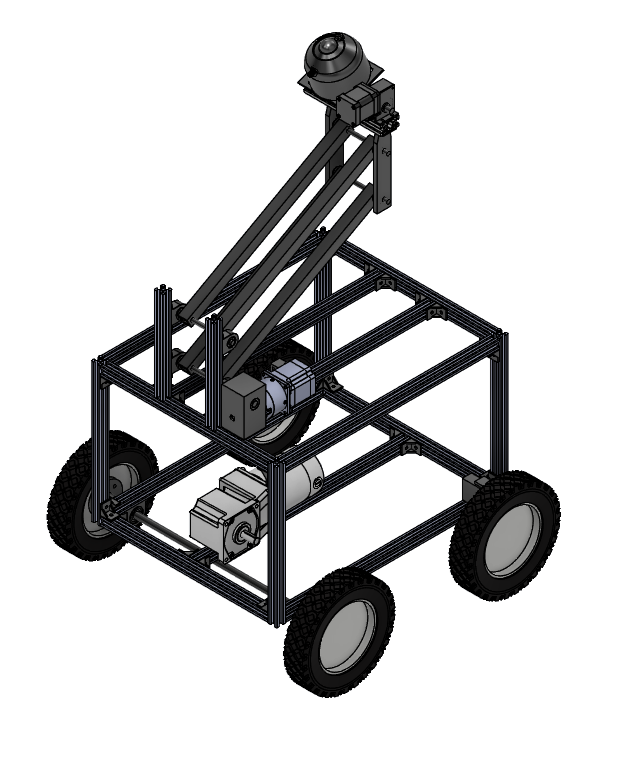
\includegraphics[width=0.6\textwidth]{Recursos/Imagenes/ImagenesDisenoMecanico/ENSAMBLAJE_GENERAL.png} \par\medskip
	
	\raggedright
	\footnotesize \textit{Nota.} Elaboración propia.
	\label{fig:CADGENERAL}
\end{figure}

% [COMPLETAR] Qué podría colocar aquí? (Talvez un párrafo de conexión entre la intro y el análisis de subsistemas, así como una explicación de por qué está ordenado así)


\end{document}